\documentclass[german]{beamer}

\mode<presentation>
{
 \usetheme{Madrid}

% \usecolortheme{crane}
 \usecolortheme{wolverine}
}

\usepackage{hyperref}

\usepackage[german]{babel}
\usepackage{times}
\usepackage[latin1,utf8]{inputenc}
\usepackage[OT2,T1]{fontenc}
\usepackage{shuffle}


% Stefan's abbreveations
\newcommand{\bq}{\begin{eqnarray*}}
\newcommand{\eq}{\end{eqnarray*}}
\newcommand{\eps}{\varepsilon}

\definecolor{MyYellowOrange}{cmyk}{0,0.5,1,0}
\newcommand{\superalert}[1]{{\color{MyYellowOrange}{#1}}}
\newtheorem*{myemptytheorem}{}

% dedicated environments
\newtheorem*{mytheorem27}{Hauptsatz der Differential- und Integralrechnung:} 

%%%%%%%%%%%%%%%%%%%%%%%%%%%%%%%%%%%%%%%%%%%%%%%%%%%%%%%%%%%%%%%%%%%%%%%%%%%%%%%%%%%%%%%%%%%%%%%%%%%%%%%%%
%%%%%%%%%%%%%%%%%%%%%%%%%%%%%%%%%%%%%%%%%%%%%%%%%%%%%%%%%%%%%%%%%%%%%%%%%%%%%%%%%%%%%%%%%%%%%%%%%%%%%%%%%
%%%%%%%%%%%%%%%%%%%%%%%%%%%%%%%%%%%%%%%%%%%%%%%%%%%%%%%%%%%%%%%%%%%%%%%%%%%%%%%%%%%%%%%%%%%%%%%%%%%%%%%%%

\title{Vektoranalysis}

\subtitle{Mathematischer Br\"uckenkurs}

\author{Stefan Weinzierl}

\institute[Uni Mainz]{Institut f\"ur Physik, Universit\"at Mainz}%

\date[WiSe 2020/21]{Wintersemester 2020/21}

\begin{document}

%%%%%%%%%%%%%%%%%%%%%%%%%%%%%%%%%%%%%%%%%%%%%%%%%%%%%%%%%%%%%%%%%%%%%%%%%%%%%%%%%%%%%%%%%%%%%%%%%%%%%%%%%
%%%%%%%%%%%%%%%%%%%%%%%%%%%%%%%%%%%%%%%%%%%%%%%%%%%%%%%%%%%%%%%%%%%%%%%%%%%%%%%%%%%%%%%%%%%%%%%%%%%%%%%%%
%%%%%%%%%%%%%%%%%%%%%%%%%%%%%%%%%%%%%%%%%%%%%%%%%%%%%%%%%%%%%%%%%%%%%%%%%%%%%%%%%%%%%%%%%%%%%%%%%%%%%%%%%

\begin{frame}
  \titlepage
\end{frame}

%%%%%%%%%%%%%%%%%%%%%%%%%%%%%%%%%%%%%%%%%%%%%%%%%%%%%%%%%%%%%%%%%%%%%%%%%%%%%%%%%%%%%%%%%%%%%%%%%%%%%%%%%
%%%%%%%%%%%%%%%%%%%%%%%%%%%%%%%%%%%%%%%%%%%%%%%%%%%%%%%%%%%%%%%%%%%%%%%%%%%%%%%%%%%%%%%%%%%%%%%%%%%%%%%%%
%%%%%%%%%%%%%%%%%%%%%%%%%%%%%%%%%%%%%%%%%%%%%%%%%%%%%%%%%%%%%%%%%%%%%%%%%%%%%%%%%%%%%%%%%%%%%%%%%%%%%%%%%

\section{Allgemeines}

\frame{\sectionpage}

% page --------------------------------------------------------------------------------------------------
\begin{frame}{Motivation}

\begin{itemize}
\item Eine \alert{gew\"ohnliche Funktion} ist beispielsweise eine Abbildung
\bq
 f & : & {\mathbb R} \rightarrow {\mathbb R},
 \nonumber \\
 x & \rightarrow & f\left(x\right).
\eq
\item Eine \alert{Funktion mehrerer Variablen} ist beispielsweise eine Abbildung
\bq
 f & : & {\mathbb R}^n \rightarrow {\mathbb R},
 \nonumber \\
 \left( x_1, ..., x_n \right) & \rightarrow & f\left( x_1, ..., x_n \right).
\eq
\item Wir betrachten nun den allgemeinen Fall und lassen nun auch einen \superalert{h\"oherdimensionalen Wertebereich} zu, beispielsweise
\bq
 \vec{f} & : & {\mathbb R}^n \rightarrow {\mathbb R}^m,
 \nonumber \\
 \left( x_1, ..., x_n \right) & \rightarrow & \vec{f}\left( x_1, ..., x_n \right).
\eq
\end{itemize}

\end{frame}

% page --------------------------------------------------------------------------------------------------
\begin{frame}{Definition}

\begin{definition}
Wir betrachten eine Abbildung, in dem der Definitionsbereich $U$ eine
offene Teilmenge des ${\mathbb R}^n$ und der Wertebereich $W$ eine Teilmenge des ${\mathbb R}^m$ ist:
\bq
 \vec{f} & : & U \rightarrow W,
 \nonumber \\
 \left( x_1, ..., x_n \right) & \rightarrow & \vec{f}\left( x_1, ..., x_n \right).
\eq
Man bezeichnet $\vec{f}$ als ein \superalert{Vektorfeld}.

Jedem Punkt $( x_1, ..., x_n) \in U$ wird ein Vektor $\vec{f} \in {\mathbb R}^m$ zugeordnet.
\end{definition}

\end{frame}

% page --------------------------------------------------------------------------------------------------
\begin{frame}{Vektorfelder}

Schreiben wir $\vec{f}$ in Komponenten
\bq
 \vec{f}\left( x_1, ..., x_n \right) & = & 
 \left( \begin{array}{c}
 f_1\left( x_1, ..., x_n \right) \\
 ... \\
 f_m\left( x_1, ..., x_n \right) \\
 \end{array} \right)
\eq
so haben wir $m$ Abbildungen
\bq
 f_j & : & U \rightarrow {\mathbb R},
 \nonumber \\
 \left( x_1, ..., x_n \right) & \rightarrow & f_j\left( x_1, ..., x_n \right).
\eq
Wir schreiben im folgenden $\vec{x}=( x_1, ..., x_n )$.

\end{frame}

% page --------------------------------------------------------------------------------------------------
\begin{frame}{Beispiele}

\begin{itemize}
\item \alert{Elektrische Felder}: Jedem Ortsvektor $\vec{x} \in {\mathbb R}^3$ wird ein Feld $\vec{E}(\vec{x})$ zugeordnet, da{\ss} das elektrische Feld
an diesem Ort angibt.

\vspace*{3mm}
\item \alert{Magnetische Felder}: Jedem Ortsvektor $\vec{x} \in {\mathbb R}^3$ wird ein Feld $\vec{B}(\vec{x})$ zugeordnet, da{\ss} das magnetische Feld
an diesem Ort angibt.

\vspace*{3mm}
\item \alert{Str\"omungsfelder}: Jedem Ortsvektor $\vec{x} \in {\mathbb R}^3$ wird ein Feld $\vec{v}(\vec{x})$ zugeordnet, da{\ss} die Geschwindigkeit
des Mediums 
an diesem Ort angibt.
(Dies kann eine str\"omende Fl\"ussigkeit sein, oder der Wind in der Atmosph\"are.)
\end{itemize}

\end{frame}

% page --------------------------------------------------------------------------------------------------
\begin{frame}{Beispiele}

\begin{example}
Wir betrachten drei Beispiele f\"ur Vektorfelder:
\bq 
 \vec{f}_1 & : & {\mathbb R}^2 \rightarrow {\mathbb R}^2,
 \nonumber \\
 & & \vec{f}_1(\vec{x}) = \left( \begin{array}{c} 1 \\ \sin x_1 \\ \end{array} \right),
 \nonumber \\
 \vec{f}_2 & : & {\mathbb R}^2 \rightarrow {\mathbb R}^2,
 \nonumber \\
 & & \vec{f}_2(\vec{x}) = \left( \begin{array}{c} x_1 \\ x_2 \\ \end{array} \right),
 \nonumber \\
 \vec{f}_3 & : & {\mathbb R}^2 \rightarrow {\mathbb R}^2,
 \nonumber \\
 & & \vec{f}_3(\vec{x}) = \left( \begin{array}{c} -x_2 \\ x_1 \\ \end{array} \right).
\eq
\end{example}

\end{frame}

% page --------------------------------------------------------------------------------------------------
\begin{frame}{Beispiel 1}

\bq
 \vec{f}_1(\vec{x}) & = & \left( \begin{array}{c} 1 \\ \sin x_1 \\ \end{array} \right)
\eq
\begin{figure}
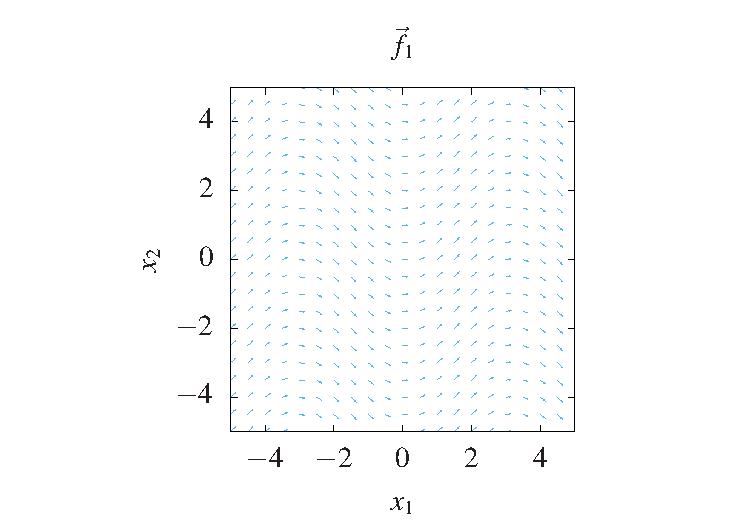
\includegraphics[scale=0.7]{f1}
\end{figure}

\end{frame}

% page --------------------------------------------------------------------------------------------------
\begin{frame}{Beispiel 2}

\bq
 \vec{f}_2(\vec{x}) & = & \left( \begin{array}{c} x_1 \\ x_2 \\ \end{array} \right)
\eq
\begin{figure}
\includegraphics[scale=0.7]{f2}
\end{figure}

\end{frame}

% page --------------------------------------------------------------------------------------------------
\begin{frame}{Beispiel 3}

\bq
 \vec{f}_3(\vec{x}) & = & \left( \begin{array}{c} -x_2 \\ x_1 \\ \end{array} \right)
\eq
\begin{figure}
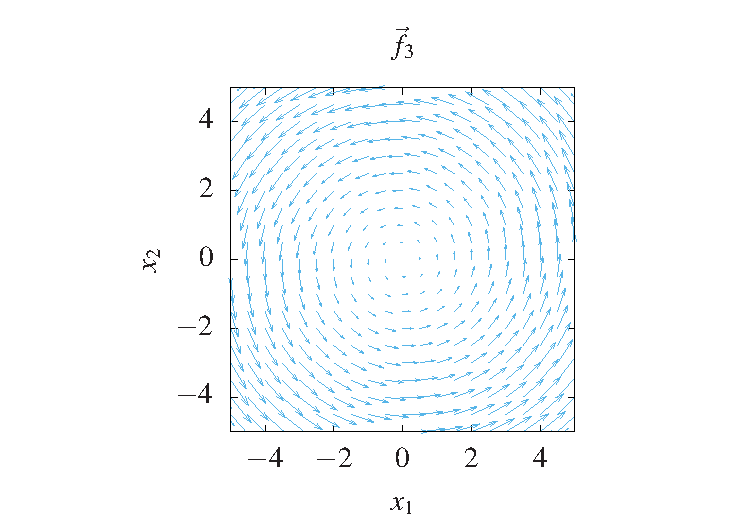
\includegraphics[scale=0.7]{f3}
\end{figure}

\end{frame}

%%%%%%%%%%%%%%%%%%%%%%%%%%%%%%%%%%%%%%%%%%%%%%%%%%%%%%%%%%%%%%%%%%%%%%%%%%%%%%%%%%%%%%%%%%%%%%%%%%%%%%%%%
%%%%%%%%%%%%%%%%%%%%%%%%%%%%%%%%%%%%%%%%%%%%%%%%%%%%%%%%%%%%%%%%%%%%%%%%%%%%%%%%%%%%%%%%%%%%%%%%%%%%%%%%%
%%%%%%%%%%%%%%%%%%%%%%%%%%%%%%%%%%%%%%%%%%%%%%%%%%%%%%%%%%%%%%%%%%%%%%%%%%%%%%%%%%%%%%%%%%%%%%%%%%%%%%%%%

\section{Die totale Ableitung}

\frame{\sectionpage}

% page --------------------------------------------------------------------------------------------------
\begin{frame}{Die totale Ableitung}

\begin{definition}
Wir bezeichnen eine Abbildung $\vec{f} : U \rightarrow {\mathbb R}^m$ als im Punkte $\vec{x}_0 \in U$
{\bf total differenzierbar}, falls es eine lineare Abbildung 
\bq
 A & : & {\mathbb R}^n \rightarrow {\mathbb R}^m,
 \nonumber \\
  \vec{x} & \rightarrow & A \vec{x},
\eq
gibt, so da{\ss} in einer Umgebung von $\vec{x}_0$ gilt:
\bq
 \vec{f}\left(\vec{x}_0+\vec{\xi}\right) & = & 
 \vec{f}\left(\vec{x}_0\right)
 + A \vec{\xi}
 + o\left(|\vec{\xi}|\right).
\eq
$A$ ist eine von $\vec{x}$ unabh\"angige $m \times n$-Matrix.
\end{definition}

\end{frame}

% page --------------------------------------------------------------------------------------------------
\begin{frame}{Die totale Ableitung}

\begin{itemize}
\item Die kleine ``o''-Schreibweise bedeutet, da{\ss} das Restglied durch eine Funktion $\vec{\varphi}(\vec{\xi})$ gegeben ist, f\"ur die 
gilt
\bq
 \lim\limits_{|\vec{\xi}|\rightarrow 0} \frac{\vec{\varphi}(\vec{\xi})}{|\vec{\xi}|} & = & \vec{0}.
\eq
Das Restglied verschwindet also schneller als der lineare Term f\"ur $|\vec{\xi}|\rightarrow 0$.

\item Die Bedingung an die totale Differenzierbarkeit bedeutet also, da{\ss} sich die Abbildung in einer hinreichend kleinen Umgebung
von $\vec{x}_0$ durch eine Konstante $\vec{f}\left(\vec{x}_0\right)$ und einen linearen Term $A \vec{\xi}$ beschreiben l\"a{\ss}t.
\end{itemize}

\end{frame}

% page --------------------------------------------------------------------------------------------------
\begin{frame}{Die Jacobi-Matrix}

Neben der totalen Differenzierbarkeit haben wir nat\"urlich noch die partiellen Ableitungen der $i$-ten Komponente $f_i$ nach
der $j$-ten Koordinate:
\bq
 \frac{\partial f_i}{\partial x_j} & = & 
 \lim\limits_{h \rightarrow 0} \frac{f_i\left(x_1,...,x_j+h,...,x_n\right)-f_i\left(x_1,...,x_j,...,x_n\right)}{h}.
\eq
Diese partiellen Ableitungen definieren eine $m \times n$ Matrix $J_{ij}$
\bq
 J_{ij}\left(\vec{x}\right) & = & \frac{\partial f_i}{\partial x_j},
 \;\;\;\;\;\;
 1 \le i \le m,
 \;\;\;
 1 \le j \le n,
\eq
die man als \superalert{Jacobi-Matrix} oder Funktional-Matrix bezeichnet.
Auch die Bezeichnung \superalert{Differential} wird verwendet, und man findet die Notation
\bq
 D\vec{f}\left(\vec{x}\right) & = & J\left(\vec{x}\right).
\eq

\end{frame}

% page --------------------------------------------------------------------------------------------------
\begin{frame}{Die totale Ableitung}

F\"ur den Zusammenhang zwischen totaler Differenzierbarkeit und partieller Differenzierbarkeit haben wir die
folgenden S\"atze:

\begin{theorem}
Sei $U \subset {\mathbb R}^n$ eine offene Teilmenge und $\vec{f} : U \rightarrow {\mathbb R}^m$ eine Abbildung,
die im Punkte $\vec{x}_0 \in U$ {\bf total differenzierbar} sei, d.h.
\bq
 \vec{f}\left(\vec{x}_0+\vec{\xi}\right) & = & 
 \vec{f}\left(\vec{x}_0\right)
 + A \vec{\xi}
 + o\left(||\vec{\xi}||\right).
\eq
Dann ist $\vec{f}$ im Punkte $\vec{x}_0$ stetig und alle Komponenten $f_j : U \rightarrow {\mathbb R}$ von $\vec{f}$
sind im Punkte $\vec{x}_0$ {\bf partiell differenzierbar} und es gilt
\bq
 \frac{\partial f_i}{\partial x_j}\left( \vec{x}_0 \right)
 & = & A_{ij}.
\eq
\end{theorem}

\end{frame}

% page --------------------------------------------------------------------------------------------------
\begin{frame}{Die totale Ableitung}

\begin{theorem}
Sei wieder $U \subset {\mathbb R}^n$ eine offene Teilmenge und $\vec{f} : U \rightarrow {\mathbb R}^m$ eine Abbildung.
Es sei weiter vorausgesetzt, da{\ss} die Abbildung $\vec{f}$ im Punkte $\vec{x}_0 \in U$ {\bf stetig partiell differenzierbar} ist,
d.h. alle partiellen Ableitungen 
\bq
\frac{\partial f_i}{\partial x_j}\left(\vec{x}_0\right)
\eq
existieren und sind stetig.
Dann ist $\vec{f}$ in $\vec{x}_0$ {\bf total differenzierbar}.
\end{theorem}

\end{frame}

% page --------------------------------------------------------------------------------------------------
\begin{frame}{Die totale Ableitung}

Wir haben also die folgenden Implikationen:
\begin{myemptytheorem}
{\footnotesize
\bq
 \mbox{stetig partiell differenzierbar }
 \Rightarrow 
 \mbox{ total differenzierbar }
 \Rightarrow
 \mbox{ partiell differenzierbar}
\eq
}
\end{myemptytheorem}

\vspace*{2mm}
Die Umkehrungen gelten im Allgemeinen nicht.

\end{frame}

%%%%%%%%%%%%%%%%%%%%%%%%%%%%%%%%%%%%%%%%%%%%%%%%%%%%%%%%%%%%%%%%%%%%%%%%%%%%%%%%%%%%%%%%%%%%%%%%%%%%%%%%%
%%%%%%%%%%%%%%%%%%%%%%%%%%%%%%%%%%%%%%%%%%%%%%%%%%%%%%%%%%%%%%%%%%%%%%%%%%%%%%%%%%%%%%%%%%%%%%%%%%%%%%%%%
%%%%%%%%%%%%%%%%%%%%%%%%%%%%%%%%%%%%%%%%%%%%%%%%%%%%%%%%%%%%%%%%%%%%%%%%%%%%%%%%%%%%%%%%%%%%%%%%%%%%%%%%%

\section{Der Nabla-Operator}

\frame{\sectionpage}

% page --------------------------------------------------------------------------------------------------
\begin{frame}{Der Gradient}

Sei $U \subset {\mathrm R}^n$ eine offene Menge und 
$\varphi : U \rightarrow {\mathbb R}$ eine partiell differenzierbare
Funktion von $n$ Variablen.

\begin{definition}
Die partiellen Ableitungen von $\varphi$ definieren ein Vektorfeld, 
welches man als den \superalert{Gradienten} von $\varphi$ bezeichnet:
\bq
 \mbox{grad} \; \varphi & : & U \rightarrow {\mathbb R}^n, 
 \nonumber \\
 & & \mbox{grad} \; \varphi\left(\vec{x}\right)
     = \left( \begin{array}{c}
              \frac{\partial \varphi\left(\vec{x}\right)}{\partial x_1} \\
              ... \\
              \frac{\partial \varphi\left(\vec{x}\right)}{\partial x_n} \\
              \end{array}
       \right).
\eq
\end{definition}
Der Gradient einer skalaren Funktion ist also ein Vektorfeld, da{\ss} in der $j$-ten Komponente die 
$j$-te partielle Ableitung enth\"alt.

\end{frame}

% page --------------------------------------------------------------------------------------------------
\begin{frame}{Der Nabla-Operator}

\begin{definition}
Der Nabla-Operator $\vec{\nabla}$ ist definiert als
\bq
 \vec{\nabla} & = & \left( \begin{array}{c}
                           \frac{\partial}{\partial x_1} \\
                           ... \\
                           \frac{\partial}{\partial x_n} \\
                           \end{array}
                    \right)
\eq
\end{definition}
Mit Hilfe des Nabla-Operators l\"a{\ss}t sich der Gradient auch wie folgt schreiben:
\bq
 \mbox{grad} \; \varphi & = & \vec{\nabla} \varphi
\eq

\end{frame}

% page --------------------------------------------------------------------------------------------------
\begin{frame}{Der Nabla-Operator}

\begin{itemize}
\item $\vec{\nabla}$ ist ein \alert{Operator}, der auf eine Gr\"o{\ss}e, wie zum Beispiel eine 
Funktion, die abgeleitet werden kann, wirkt.
Man sollte diese Gr\"o{\ss}e daher immer mitangeben. 

\item Mathematische Beziehungen, in denen die
Gr\"o{\ss}e auf die ein Operator wirkt fehlt, machen nur Sinn, wenn sie f\"ur alle
m\"oglichen Gr\"o{\ss}en des Problems (wie zum Beispiel f\"ur alle Testfunktionen) gelten.
\end{itemize}

\end{frame}

% page --------------------------------------------------------------------------------------------------
\begin{frame}{Der Nabla-Operator}

\begin{example}
Wir betrachten die Funktion
\bq
 \varphi & : & {\mathbb R}^3 \rightarrow {\mathbb R},
 \nonumber \\
 & & \varphi\left(\vec{x}\right) = x_1^2 + x_2^2 + x_3^2.
\eq
Wir erhalten f\"ur den Gradienten
\bq
 \mbox{grad}\; \varphi\left(\vec{x}\right)
 & = & \vec{\nabla} \varphi\left(\vec{x}\right)
 =
 \left( \begin{array}{c}
  2 x_1 \\ 2 x_2 \\ 2 x_3 \\
 \end{array} \right).
\eq
\end{example}

\end{frame}

% page --------------------------------------------------------------------------------------------------
\begin{frame}{Minima und Maxima}

\begin{itemize}
\item Wir hatten bereits gesehen, da{\ss} eine notwendige Bedingung f\"ur das Vorliegen eines lokalen Maximums bzw.
eines lokalen Minimums im Punkte $\vec{x}_0$ das Verschwinden aller partiellen Ableitungen in diesem Punkte ist.
\item Das Verschwinden aller partiellen Ableitungen ist gleichbedeutend mit der Aussage
\bq
 \vec{\nabla} \varphi\left(\vec{x}_0\right) & = & \vec{0},
\eq
d.h. der Gradient verschwindet.
\end{itemize}

\end{frame}

% page --------------------------------------------------------------------------------------------------
\begin{frame}{Quiz}

\bq
 \varphi & : & {\mathbb R}^2 \rightarrow {\mathbb R},
 \nonumber \\
 & & \varphi\left(\vec{x}\right) = x_1 x_2
\eq
\bq
 \vec{\nabla} \varphi\left(\vec{x}\right)
 & = & ?
\eq
\begin{columns}[b]
\begin{column}{5cm}
\begin{description}
\item{(A)} $\left(\begin{array}{c} 0 \\ 0 \\ \end{array} \right)$
\item{(C)} $\left(\begin{array}{c} x_1 \\ x_2 \\ \end{array} \right)$
\end{description}
\end{column}
\begin{column}{5cm}
\begin{description}
\item{(B)} $\left(\begin{array}{c} 1 \\ 1 \\ \end{array} \right)$
\item{(D)} $\left(\begin{array}{c} x_2 \\ x_1 \\ \end{array} \right)$
\end{description}
\end{column}
\end{columns}

\end{frame}

% page --------------------------------------------------------------------------------------------------
\begin{frame}{Die Divergenz}

\begin{definition}
Sei $U \subset {\mathrm R}^n$ eine offene Menge und 
$\vec{f} : U \rightarrow {\mathbb R}^n$ eine partiell differenzierbares Vektorfeld.
Wir definieren die \superalert{Divergenz} dieses Vektorfeldes als eine skalare Funktion der $n$ Variablen
\bq
 \mbox{div}\; \vec{f} & : & U \rightarrow {\mathbb R},
\eq
die durch
\bq
 \mbox{div}\; \vec{f}\left(\vec{x}\right) & = & 
  \sum\limits_{j=1}^n \frac{\partial f_j\left(\vec{x}\right)}{\partial x_j}
\eq
gegeben ist.
Mit Hilfe des Nabla-Operators schreibt man auch oft
\bq
 \mbox{div}\; \vec{f}\left(\vec{x}\right) & = & 
 \vec{\nabla} \cdot \vec{f}\left(\vec{x}\right).
\eq
\end{definition}

\end{frame}

% page --------------------------------------------------------------------------------------------------
\begin{frame}{Die Divergenz}

\begin{example}
Wir betrachten das Vektorfeld
\bq
 \vec{f} & : & {\mathbb R}^3 \rightarrow {\mathbb R}^3,
 \nonumber \\
 & & \vec{f}\left(\vec{x}\right)
 =
 \left( \begin{array}{c}
  x_1^2 + x_2 \\ 3 x_2 - x_1 \\ 5 x_3 + 7 x_2 \\
 \end{array} \right).
\eq
Wir erhalten f\"ur die Divergenz
\bq
 \mbox{div}\; \vec{f}\left(\vec{x}\right) & = & 
 \vec{\nabla} \cdot \vec{f}\left(\vec{x}\right)
 =
 2 x_1 + 3 + 5 = 2 x_1 + 8.
\eq
\end{example}

\end{frame}

% page --------------------------------------------------------------------------------------------------
\begin{frame}{Die Divergenz}

\begin{example}
Es ist auch interessant die Divergenz der drei eingangs gezeigten Vektorfelder zu berechnen.
Man findet:
\bq
 \mbox{div} \; \vec{f}_1(\vec{x})
 & = &
 \vec{\nabla} \cdot \vec{f}_1(\vec{x})
 = 
 \frac{\partial}{\partial x_1} 1 + \frac{\partial}{\partial x_2} \sin x_1 = 0,
 \nonumber \\
 \mbox{div} \; \vec{f}_2(\vec{x})
 & = &
 \vec{\nabla} \cdot \vec{f}_2(\vec{x})
 = 
 \frac{\partial}{\partial x_1} x_1 + \frac{\partial}{\partial x_2} x_2 = 2,
 \nonumber \\
 \mbox{div} \; \vec{f}_3(\vec{x})
 & = &
 \vec{\nabla} \cdot \vec{f}_3(\vec{x})
 = 
 \frac{\partial}{\partial x_1} \left( - x_2 \right) + \frac{\partial}{\partial x_2} x_1 = 0.
\eq
Von diesen drei Beispielen hat also nur $\vec{f}_2$ eine nicht-verschwindende Divergenz.

Die Divergenz beschreibt die {\bf Quellen} und {\bf Senken} eines Vektorfeldes.
\end{example}

\end{frame}

% page --------------------------------------------------------------------------------------------------
\begin{frame}{Quiz}

\bq
 \vec{f} & : & {\mathbb R}^2 \rightarrow {\mathbb R}^2,
 \nonumber \\
 & & \vec{f}\left(\vec{x}\right)
 =
 \left( \begin{array}{c}
  x_1 x_2 \\ 3 x_1 x_2 \\
 \end{array} \right).
\eq
\bq
 \vec{\nabla} \cdot \vec{f}\left(\vec{x}\right)
 & = & ?
\eq
\begin{description}
\item{(A)} $4$
\item{(B)} $3 x_1 + x_2$
\item{(C)} $x_1 + 3 x_2$
\item{(D)} $4 x_1 x_2$
\end{description}

\end{frame}

% page --------------------------------------------------------------------------------------------------
\begin{frame}{Der Laplace-Operator}

Wir betrachten noch die folgende Kombination von Gradient und Divergenz:

\vspace*{2mm}
Sei $U \subset {\mathrm R}^n$ eine offene Menge und 
$\varphi : U \rightarrow {\mathbb R}$ eine zweimal stetig partiell differenzierbare
Funktion von $n$ Variablen.

\vspace*{2mm}
Wir wenden erst den Gradienten auf $\varphi$ an, und dann die Divergenz auf das resultierende Vektorfeld.
Wir erhalten somit wieder eine skalare Funktion:
\begin{definition}
\bq
 \Delta \varphi & : & U \rightarrow {\mathbb R},
 \nonumber \\
 & & \Delta \varphi\left(\vec{x}\right) = \mbox{div} \; \mbox{grad} \; \varphi\left(\vec{x}\right)
 = \sum\limits_{j=1}^n \frac{\partial^2 \varphi\left(\vec{x}\right)}{\partial x_j^2}.
\eq
\end{definition}

\end{frame}

% page --------------------------------------------------------------------------------------------------
\begin{frame}{Der Laplace-Operator}

\begin{myemptytheorem}
Mit Hilfe des Nabla-Operators k\"onnen wir wieder schreiben:
\bq
 \Delta \varphi\left(\vec{x}\right) & = & \vec{\nabla} \cdot \vec{\nabla} \varphi\left(\vec{x}\right).
\eq
\end{myemptytheorem}
\begin{definition}
Wir bezeichnen mit
\bq
 \Delta & = & \vec{\nabla} \cdot \vec{\nabla} 
 = \sum\limits_{j=1}^n \frac{\partial^2}{\partial x_j^2}
\eq
den \superalert{Laplace-Operator}.
\end{definition}

\end{frame}

% page --------------------------------------------------------------------------------------------------
\begin{frame}{Der Laplace-Operator}

\begin{example}
Wir betrachten die Funktion
\bq
 \varphi & : & {\mathbb R}^3 \rightarrow {\mathbb R},
 \nonumber \\
 & & \varphi\left(\vec{x}\right) = x_1^2 + x_2^2 + x_3^2.
\eq
Wir hatten bereits den Gradienten berechnet:
{\footnotesize
\bq
 \mbox{grad}\; \varphi\left(\vec{x}\right)
 & = & \vec{\nabla} \varphi\left(\vec{x}\right)
 =
 \left( \begin{array}{c}
  2 x_1 \\ 2 x_2 \\ 2 x_3 \\
 \end{array} \right).
\eq
}

\vspace*{-3mm}
Die Anwendung des Laplace-Operators ergibt
\bq
 \Delta \varphi\left(\vec{x}\right)
 & = &
 \vec{\nabla} \cdot  
 \left( \begin{array}{c}
  2 x_1 \\ 2 x_2 \\ 2 x_3 \\
 \end{array} \right)
 \; = \;
 2 + 2 + 2 \; = \; 6.
\eq

\end{example}

\end{frame}

%%%%%%%%%%%%%%%%%%%%%%%%%%%%%%%%%%%%%%%%%%%%%%%%%%%%%%%%%%%%%%%%%%%%%%%%%%%%%%%%%%%%%%%%%%%%%%%%%%%%%%%%%
%%%%%%%%%%%%%%%%%%%%%%%%%%%%%%%%%%%%%%%%%%%%%%%%%%%%%%%%%%%%%%%%%%%%%%%%%%%%%%%%%%%%%%%%%%%%%%%%%%%%%%%%%
%%%%%%%%%%%%%%%%%%%%%%%%%%%%%%%%%%%%%%%%%%%%%%%%%%%%%%%%%%%%%%%%%%%%%%%%%%%%%%%%%%%%%%%%%%%%%%%%%%%%%%%%%

\section{Vektorfelder in drei Dimensionen}

\frame{\sectionpage}

% page --------------------------------------------------------------------------------------------------
\begin{frame}{Vektorfelder in drei Dimensionen}

Wir betrachten noch den Spezialfall von Vektorfeldern in drei Dimensionen:
\bq
 \vec{A} & : & {\mathbb R}^3 \rightarrow {\mathbb R}^3.
\eq

\end{frame}

% page --------------------------------------------------------------------------------------------------
\begin{frame}{Die Rotation}

\begin{definition}
Hier k\"onnen wir noch eine weitere Operation einf\"uhren, die man als \superalert{Rotation} bezeichnet und wie
folgt definiert ist:
\bq
 \mbox{rot} \; \vec{A} & : & {\mathbb R}^3 \rightarrow {\mathbb R}^3,
 \nonumber \\
 & &\mbox{rot} \; \vec{A}\left(\vec{x}\right) =
    \left( \begin{array}{c}
      \frac{\partial A_3\left(\vec{x}\right)}{\partial x_2} - \frac{\partial A_2\left(\vec{x}\right)}{\partial x_3} \\
      \frac{\partial A_1\left(\vec{x}\right)}{\partial x_3} - \frac{\partial A_3\left(\vec{x}\right)}{\partial x_1} \\
      \frac{\partial A_2\left(\vec{x}\right)}{\partial x_1} - \frac{\partial A_1\left(\vec{x}\right)}{\partial x_2} \\
           \end{array}
    \right).
\eq
\end{definition}
\begin{myemptytheorem}
Mit Hilfe des Nabla-Operators und des Kreuzproduktes l\"a{\ss}t sich dies auch schreiben als
\bq
 \mbox{rot} \; \vec{A}\left(\vec{x}\right) & = & \vec{\nabla} \times \vec{A}\left(\vec{x}\right).
\eq
\end{myemptytheorem}

\end{frame}

% page --------------------------------------------------------------------------------------------------
\begin{frame}{Die Rotation}

\begin{example}
Sei
\bq
 \vec{A} & : & {\mathbb R}^3 \rightarrow {\mathbb R}^3,
 \nonumber \\
 & & \vec{A}\left(\vec{x}\right) =
     \left( \begin{array}{c} -x_2 \\ x_1 \\ 0 \\ \end{array} \right).
\eq
Dann ist
\bq
 \mbox{rot} \; \vec{A}\left(\vec{x}\right) & = & \vec{\nabla} \times \vec{A}\left(\vec{x}\right)
 = \left( \begin{array}{c}
    0 \\ 0 \\ 2 \\
   \end{array} \right)
\eq
\end{example}

\end{frame}

% page --------------------------------------------------------------------------------------------------
\begin{frame}{Die Rotation}

\begin{example}
Kehren wir nocheinmal zu den eingangs diskutierten Vektorfeldern zur\"uck. 

\vspace*{4mm}
Diese Vektorfelder sind
Abbildungen von ${\mathbb R}^2$ nach ${\mathbb R}^2$, daher ist die Operation der Rotation nicht unmittelbar darauf anwendbar.

\vspace*{4mm}
Wir k\"onnen aber trotzdem f\"ur ein Vektorfeld $\vec{f}=(f_1,f_2)$ die anti-symmetrische Ableitung
\bq
 \frac{\partial}{\partial x_1} f_2 - \frac{\partial}{\partial x_2} f_1
\eq
betrachten.
\end{example}

\end{frame}

% page --------------------------------------------------------------------------------------------------
\begin{frame}{Die Rotation}

\begin{example}
Wir finden:
\bq
 \frac{\partial}{\partial x_1} f_{12} - \frac{\partial}{\partial x_2} f_{11}
 & = &
 \frac{\partial}{\partial x_1} \sin x_1 - \frac{\partial}{\partial x_2} 1
 = \cos(x_1),
 \nonumber \\
 \frac{\partial}{\partial x_1} f_{22} - \frac{\partial}{\partial x_2} f_{21}
 & = &
 \frac{\partial}{\partial x_1} x_2 - \frac{\partial}{\partial x_2} x_1
 = 0,
 \nonumber \\
 \frac{\partial}{\partial x_1} f_{32} - \frac{\partial}{\partial x_2} f_{31}
 & = &
 \frac{\partial}{\partial x_1} x_1 - \frac{\partial}{\partial x_2} \left( - x_2 \right)
 = 2.
\eq
Die Rotation beschreibt die {\bf Wirbel} eines Vektorfeldes.
\end{example}

\end{frame}

% page --------------------------------------------------------------------------------------------------
\begin{frame}{Rotation eines Gradientenfeldes}

\begin{theorem}
Sei $U \subset {\mathrm R}^3$ eine offene Menge und 
$\varphi : U \rightarrow {\mathbb R}$ eine zweimal stetig partiell differenzierbare
Funktion. Dann
\bq
 \mbox{rot} \; \mbox{grad} \; \varphi & = & 0,
 \nonumber \\
 \vec{\nabla} \times \left( \vec{\nabla} \varphi \right) & = & 0.
\eq
\end{theorem}
\begin{proof}
Wir betrachten die erste Komponente von $\mbox{rot} \; \mbox{grad} \; \varphi$:
\bq
 \frac{\partial}{\partial x_2} \frac{\partial}{\partial x_3} \varphi 
 -
 \frac{\partial}{\partial x_3} \frac{\partial}{\partial x_2} \varphi 
 & = & 0.
\eq
Gleiches gilt f\"ur die anderen Komponenten. 

\vspace*{2mm}
Ein Gradientenfeld ist also rotationsfrei.
\end{proof}

\end{frame}

% page --------------------------------------------------------------------------------------------------
\begin{frame}{Divergenz eines Rotationsfeldes}

\begin{theorem}
Sei $U \subset {\mathrm R}^3$ eine offene Menge und 
$\vec{f} : U \rightarrow {\mathbb R}^3$ eine zweimal stetig partiell differenzierbares Vektorfeld.
Dann
\bq
 \mbox{div} \; \mbox{rot} \; \vec{f} & = & 0,
 \nonumber \\
 \vec{\nabla} \cdot \left( \vec{\nabla} \times \vec{f} \right) & = & 0.
\eq
\end{theorem}
\begin{proof}
{\scriptsize
\bq
 \vec{\nabla} \cdot \left( \vec{\nabla} \times \vec{f} \right) 
 & = &
 \frac{\partial}{\partial x_1} \left( \frac{\partial}{\partial x_2} f_3 - \frac{\partial}{\partial x_3} f_2 \right)
 +
 \frac{\partial}{\partial x_2} \left( \frac{\partial}{\partial x_3} f_1 - \frac{\partial}{\partial x_1} f_3 \right)
 +
 \frac{\partial}{\partial x_3} \left( \frac{\partial}{\partial x_1} f_2 - \frac{\partial}{\partial x_2} f_1 \right)
 \nonumber \\
 & = & 0.
\eq
}

\vspace*{2mm}
Ein Rotationsfeld ist also divergenzfrei.
\end{proof}

\end{frame}

%%%%%%%%%%%%%%%%%%%%%%%%%%%%%%%%%%%%%%%%%%%%%%%%%%%%%%%%%%%%%%%%%%%%%%%%%%%%%%%%%%%%%%%%%%%%%%%%%%%%%%%%%
%%%%%%%%%%%%%%%%%%%%%%%%%%%%%%%%%%%%%%%%%%%%%%%%%%%%%%%%%%%%%%%%%%%%%%%%%%%%%%%%%%%%%%%%%%%%%%%%%%%%%%%%%
%%%%%%%%%%%%%%%%%%%%%%%%%%%%%%%%%%%%%%%%%%%%%%%%%%%%%%%%%%%%%%%%%%%%%%%%%%%%%%%%%%%%%%%%%%%%%%%%%%%%%%%%%

% page --------------------------------------------------------------------------------------------------
\begin{frame}{Zum Schluss des Br\"uckenkurses:}

\begin{center}
{\huge
Viel Erfolg in Ihrem Studium!
}
\end{center}

\end{frame}

% page --------------------------------------------------------------------------------------------------
\begin{frame}

\end{frame}

\end{document}
